\chapter{Ausgabemethoden}
\label{cha:Ausgabe}

Im Kapitel~\ref{cha:Eingabe} wurden alternative Eingabemethoden zur Interaktion Hands-Free näher erläutert. Dieses Kapitel befasst sich mit Ausgabemethoden, die aber nicht zwingend an ihre Eingabemethoden gebunden sind. So gibt es nicht nur bei Systemen, die über die Sprache gesteuert werden, ein akustisches Feedback, sondern auch bei Systemen, die beispielsweise über die Augen oder den Mund gesteuert werden. 

\section{Auditiver Output}

Eine mögliche Form, wie ein Computer Feedback geben kann, funktioniert über die Sprache. Während bei der Spracheingabe die gesprochene Sprache von einem System in einen Befehl umgewandelt wird, gibt bei der Sprachausgabe der Computer die Informationen in Form von Sprache aus. Da die Sprachausgabe von Menschen gehört und automatisch bewertet wird, ist es wichtig, dass die Sprache von hoher Qualität ist, also möglichst real erscheint. 

	%abbildung 1
	\begin{figure}
	\centering
	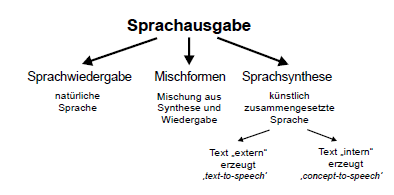
\includegraphics[width=.7\textwidth]{sprachausgabe_overview}
	\caption{Unterteilung der Sprachausgabe \cite{FellbaumSprache}.}
	\label{fig:SprachausgabeOverview}
	\end{figure}
	
\newpage
Wie in Abb.~\ref{fig:SprachausgabeOverview} dargestellt gibt es zwei unterschiedliche Ansätze, wie der Computer den Text in Sprache umwandeln kann:
\begin{itemize}
      \item Sprachwiedergabe
      \item Sprachsynthese
\end{itemize}
\newline \newline
%SPRACHWIEDERGABE
Bei der Sprachwiedergabe werden Sprachsignale ausgegeben, die zuvor aufgenommen und abgespeichert worden sind. Der Umfang an möglichen akustischen Meldungen also an Wörtern ist aus diesem Grund an die Anzahl der Aufnahmen gebunden und daher begrenzt. Da die Signale bzw. Wörter von einer realen Person eingesprochen wurden, weißt diese Methode eine sehr hohen Sprachqualität auf \cite{KaufmannPfisterSprache}.

Es gibt unterschiedliche Methoden bzw. Verfahren, wie die Sprachwiedergabe im Detail funktioniert. Zusammenfassend werden die Wörter zu Beginn von einer Person eingesprochen, bearbeitet und abgespeichert. Die einzelnen Sprachelemente werden anschließend adressiert, sodass sie vom System später leicht gefunden werden können. Wenn der Computer nun einen Text vorlesen soll, wird im System anhand der gespeicherten Adressen die einzelnen Wörter bzw. Phrasen herausgesucht und verwendet \cite{FellbaumSprache}.
\newline \newline
%SPRACHSYNTHESE
Im Gegensatz zur Sprachwiedergabe wird bei der Sprachsynthese das Ziel verfolgt alle möglichen Wortkombinationen in ein Sprachsignal umwandeln zu können. Da die Grundlage für die Wörter bzw. Ausgabe nicht von einer Person eingesprochen werden, sondern die einzelnen Wörter mit ihrer Betonung künstlich erzeugt werden müssen, sinkt dadurch die Sprachqualität und das Endergebnis gleicht oft mehr einer Computerstimme als der einer menschlichen. 

Bei der Sprachsynthese werden Silben aus verschiedenen Wörtern einzeln abgespeichert und so alle beliebigen Kombinationen zusammengesetzt. Im Anschluss werden Betonungen, Lautstärke und Geschwindigkeit hinzugefügt bzw. angepasst. Bei der sogenannten textgesteuerte Sprachsynthese (‚text-to-speech‘) ist dem System der eigentliche Inhalt des Textes nicht bekannt. Es können aber nicht nur einzelne Sätze bzw. ganze Texte verarbeitet werden, sondern auch Konzepte können vom System in Signale umgewandelt werden (,concept-to-speech'). Hier kann das System einen Text eigenständig kreieren, wenn das Konzept bzw. der Inhalt bekannt ist \cite{FellbaumSprache}.
\newline \newline
%zitat Fellbaum
Laut Fellbaum \cite{FellbaumSprache} besteht die größte Herausforderung der Sprachsynthese darin, die Stimme noch natürlicher und nicht roboterähnlich wirken zu lassen. Daher sind Mischformen zwischen Sprachwiedergabe und Sprachsynthese in der Praxis üblich. 

\section{Haptischer Ausgabe}
%TODO what to write here
%definition haptik
Es gibt verschiedene Arten von haptischem Feedback:
\begin{itemize}
      \item Thermales Feedback (Wärme)
      \item Vibration
			\item Feedback durch ein haptisches Steuerungselement
\end{itemize}

\section{Visueller Ausgabe}
%TODO what to write here
Arten von visuellem Ausgabe:
\begin{itemize}
      \item in Form von Text oder Mediaelementen am Bildschirm
      \item Grafiken/Symbole (Häckchen oder Kreuze)
\end{itemize}




